% Author Josué Galeano
% Galileo University

\documentclass[12pt]{article}

%paquetes - begin
\usepackage[left=2cm, right=2cm, top=2.7cm, bottom=2.7cm]{geometry}
\usepackage{graphicx}
\usepackage{xcolor}
\usepackage{titlesec}
\usepackage[utf8]{inputenc} % Tildes
\usepackage[spanish]{babel} % Language
\usepackage{babelbib} % Bibliografia español
\usepackage{amssymb}
\usepackage{amsmath, amsthm, amsfonts}
\usepackage[all]{xy}
\usepackage{fancyhdr}
\usepackage{lastpage}
\usepackage{float}
\usepackage{url}
\usepackage{hyperref}
\usepackage{makecell}%To keep spacing of text in tables
\usepackage{utilidades}
\setcellgapes{4pt}
%paquetes - end

%Configuraciones - begin
\newcommand{\docOwner}{Estadística Matemática}

\graphicspath{{img/}}
\titleformat{\section}{\normalfont \Large \bfseries}
{\hspace*{-1cm}\color{white}\thesection}{2.3ex plus .2ex}{} 
\titlespacing{\subsection}{2em}{*1}{*1}
\titleformat{\subsection}{\normalfont \large \bfseries}
{\hspace*{-1cm}\color{white}\thesection}{2.3ex plus .2ex}{} 
\renewcommand{\arraystretch}{1.5}
\newcommand{\enumtab}[2]{\Large $\bullet$ #1. & \Large $\bullet$ #2.\\}
\pagestyle{fancy}
\fancyhf{}
\rhead{\docOwner}
\lhead{Universidad Galileo}
\rfoot{Pág. \thepage \hspace*{.25mm} de \pageref{LastPage}}
\lfoot{\LaTeX}
\hypersetup{colorlinks=true, linkcolor=black, urlcolor=blue}
\decimalpoint
%Configuraciones - end

\usepackage{tabularx}
\begin{document}
	%%%%%% Caratula para documentos %%%%%%%

\def\title{ %titulo
	Distribuciones de probabilidad
}
\def\logo{logo} %nombre del logo (si está en img). IMPORTANTE: no deje espacios!!!
\def\date{ %fecha
	Guatemala, 10 de mayo de 2020
}
\def\subtitle{ %subtitulos o nombres de catedráticos
	Dr. Jorge Samayoa\\
	Ing. Preng Biba
}
\def\profile{ %información personal
	Josu\'e Benyamin Isa\'i Galeano Morales\\
	Carnet: 18002955\\
	II - FISICC
}

\begin{titlepage}
	\vspace*{-1.5cm}
	\begin{flushleft}
		
\includegraphics[scale=.6]{\logo}
	\end{flushleft}
	\vspace*{\fill}
	\begin{center}
		\textbf{\Huge \title} \\ %titulo
		\vspace{.3in}
		{\huge \docOwner}\\
		\vspace{.2in}
		{\Large \subtitle}
	\end{center}
	\vspace*{\fill}
	
	\begin{flushright}
		\large
		\profile
	\end{flushright}
	\begin{center}
		\emph{\date}
	\end{center}
\end{titlepage}
	\newcommand{\overview}[9]{
	\begin{tabularx}{\textwidth}{|c|X|}
		\hline
		\multicolumn{2}{|c|}{\large\textbf{Resumen}}\\
		\hline
		\textbf{Variable Aleatoria}&#1\\
		\hline
		\textbf{Func. de densidad de probabilidad}&#2\\
		\hline
		\textbf{Func. de distribución acumulada}&#3\\
		\hline
		\textbf{Valor Esperado}&#4\\
		\hline
		\textbf{Varianza}&#5\\
		\hline
		\textbf{Aplicaciones}&#6\\
		\hline
		\textbf{Gráf. de la función de densidad}&\multicolumn{1}{m{#9}|}{#7}\\
		\hline
		\textbf{Ejemplo}&#8\\
		\hline
		
	\end{tabularx}
}
	\tableofcontents
	
	\newpage	
	
	\def\arraystretch{1.6}
		
	\section{Distribuciones Discretas}
	\subsection{Distribución de Bernoulli}
	
	Es una distribución que sólo toma 2 valores, p cuando está evaluada en 1 y q cuando se evalúa en 0, la variable aleatoria en esta distribución cuenta la cantidad de éxitos, como está restringido su dominio en 0 y 1 significa que sólo puede decir cuanto es la probabilidad de que se falle o se tenga éxito, la distribución \textit{Binomial} se basa en n pruebas independientes de la \textbf{distribución de Bernoulli}.\\
	
	\hspace*{-.7cm}\overview{Cuenta la cantidad de éxitos}{$f(x)=p^x(1-q)^{1-x}$, $x\in\{0,1\}$}{$f(0<x)=0,\quad f(0\leq x<1)=q,\quad f(x\ge1)=1$}{$E(X)=p$}{\textit{VAR}$(X)=pq$}{Buscar la probabilidad cuando sólo se hace una prueba}{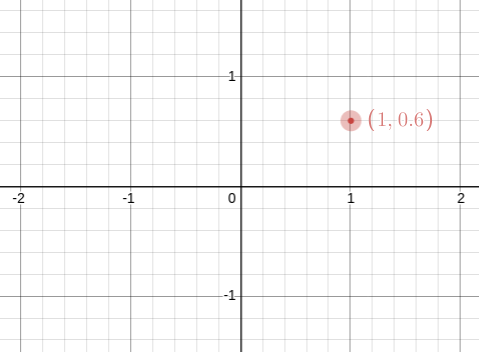
\includegraphics[scale=.5]{bernoulli}}{
		Suponemos que somos muy fans de un corredor de una competición ciclista en la cual solo compiten dos corredores. Queremos apostar a que ese corredor gana.
		$$p=0.5,\quad q=1-p=0.5$$
		Entonces, si gana será un resultado “éxito” y si pierde será un resultado “no éxito”. 
	}{9cm}
	
	\subsection{Distribución Beta-Binomial}
	\hspace*{-.7cm}\overview{Número de éxitos, pero estos no tienen la misma probabilidad}{$f(x)={n \choose x}\frac{B(x+\alpha, n-x+\beta)}{B(\alpha, \beta)}$, donde $B(\alpha, \beta)$, es la función Beta}{$f(0\leq x<n)={n \choose x}\frac{B(x+\alpha, n-x+\beta)}{B(\alpha, \beta)}$ ${}_3F_2(a,b,x),$ esta es la función hipergeométrica generalizada, $ f(0<x)=0,\; f(x\ge1)=1$}{$E(X)=\displaystyle\frac{n\alpha}{\alpha+\beta}$}{\small\textit{VAR}$(X)=\displaystyle\frac{n\alpha(\alpha+\beta+n)}{(\alpha+\beta)^2(\alpha+\beta+1)}$}{utilizada cuando se tiene condiciones similares que la \textit{binomial} pero con probabilidad variable.}{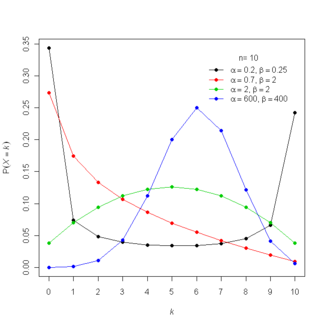
\includegraphics[scale=0.5]{beta}}{
		Se quiere obtener la pdf de una variable aleatoria que cuenta el número de niños entre los primeros 12 jóvenes, de familias con 13 personas con una cantidad de 6115 familias para muestrear. La distribución binomial se queda muy por detrás de la beta-binomial ya no se dan más restricciones como para definir una probabilidad de éxito estática. datos: 
		$$boys\quad0\quad\quad\,1\quad\quad\,2\quad\quad\,3\quad\quad\,4\quad\quad\,5\quad\quad\,6\quad\,...$$
		$$familias\quad3\quad 24\quad 104\quad 286 \quad 	670 \quad	1033 \quad1343\quad\,...$$
	}{9cm}

	\subsection{Distribución de Rademacher}
	\hspace*{-.7cm}\overview{Nada en específico}{$f(x)=0.5\;si\;x \in\{1,2\},\,0$ en otro caso}{$f(-1<x)=0,\; f(-1\leq x<1)=0.5,\; f(x\ge1)=1$}{$E(X)=0$}{\textit{VAR}$(X)=1$}{utilizada en bootstrapping, que es la práctica de estimar propiedades de un estimador}{\includegraphics[scale=0.8]{rademacher}}{
		Simon Newcomb la usó cuando obtuvo el conjunto de datos sobre la velocidad de la luz para la modelación de la desviación típica y mediana las cuales diferían de sus distribuciones muestrales.
		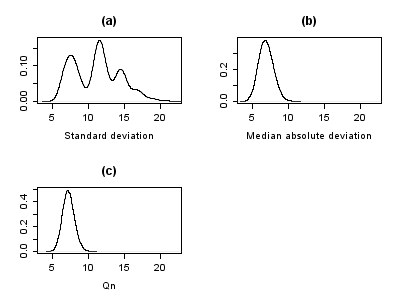
\includegraphics[scale=0.4]{dis}
	}{9cm}

	\subsection{Distribución Uniforme discreta}
		\def\arraystretch{2}
		
		Esta es equivalente a la \textbf{\textit{Distribución normal continua}} sólo que con un número discreto de casos, por la forma en que está definida cada valor de la variable aleatoria está 1 entero de distancia del siguiente y el anterior.\\
		
		
	\hspace*{-.7cm}\overview{modela eventos con la misma probabilidad}{$f(x)=1/n$}{$F(x)=\displaystyle\frac{x-a+1}{n}$}{$E(X)=\displaystyle\frac{a+b}{2}$}{\textit{VAR}$(X)=\displaystyle\frac{(b-a+1)^2-1}{12}$}{Para modelar la probabilidad de n resultados equi-probables (con la misma probabilidad de ocurrencia)}{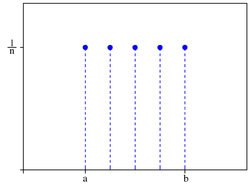
\includegraphics[scale=.5]{unifdis}}{
		se tira un dado balanceado, la probabilidad de que caiga un número en específico es de 1/6, cuando se tira una moneda balanceada, la probabilidad es de 1/2
	}{9cm}

	\subsection{Distribución Binomial Negativa}
	\def\arraystretch{2}
	
	Es una distribución compuesta de otras como las distribución de pascal (Geométrica) y la Binomial.\\
	
	
	\hspace*{-.7cm}\overview{modela la cantidad de pruebas necesarias para obtener un número predefinido de r éxitos}{$f(x)={\displaystyle {x+r+1 \choose x}}(1-p)^rp^x$}{$F(x)=1-I_p(x+1,r)$, que es la función beta incompleta}{$E(X)=\displaystyle\frac{pr}{1-p}$}{\textit{VAR}$(X)=\displaystyle\frac{pr}{(1-p)^2}$}{Cuando se necesita calcular cual es la probabilidad que ocurra r cantidad éxitos si se realizan dicha cantidad de pruebas.)}{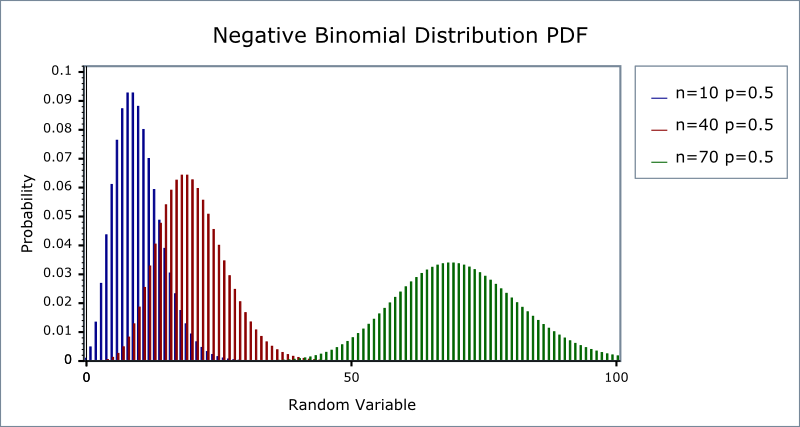
\includegraphics[scale=.4]{Negbinomial}}{
		Se requiere que Pat Collis venda golosinas para recaudar dinero para la excursión de 6to grado. Hay treinta casas en el vecindario, y no se supone que Pat regrese a casa hasta que se hayan vendido cinco barras de chocolate. Entonces el niño va de puerta en puerta y vende golosinas. En cada casa, hay una probabilidad de 0.6 de vender una barra de chocolate y una probabilidad de 0.4 de no vender nada.
		
		Como se puede observar se busca que se vendan 5 barras (éxitos).
	}{9cm}

	
	\section{Distribuciones Continuas}
	
	\subsection{Distribución Triangular}
	
	\overview{
		mide eventos donde se desconocen muchos datos.
	}{
		$f(x)=0,\,x<a\quad f(x)=\frac{2(x-a)}{(b-a)(c-a)},\, a\leq x < c,\quad f(x)=\frac{2}{b-a},\, x=c, \quad f(x)=\frac{2(b-x)}{(b-a)(b-c)},\, c< x \leq b,\quad f(x)=0,\, b < x $
	}{
		$F(x)=0,\,x\leq a\quad F(x)=\frac{(x-a)^2}{(b-a)(c-a)},\, a<x \leq c,\quad F(x)=1-\frac{(b-x)^2}{(b-a)(b-c)},\, c<x<b, \quad F(x)=1,\, b \leq x $
	}{
		$$\frac{a+b+c}{3}$$
	}{
		$$\frac{a^2+b^2+c^2-ab-ac-bc}{18}$$
	}{
		habitualmente empleado para descripción subjetiva de  poblaciones con cantidad limitada de datos
	}{
		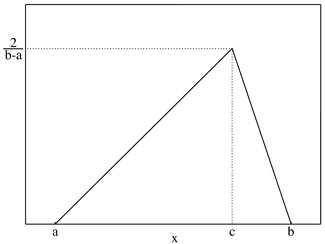
\includegraphics[scale=.5]{triangular}
	}{
		se sabe que los efectos secundarios de ampliar una imagen con ancho 128px se distribuye triangular con $c = 35$ (la moda) y extremos $a=0$ y $b=128$
	}{9cm}
	
	\Note{a, b son los extremos de la distribución y c es la moda.}
	
	\subsection{Distribución F}
	
	\overview{
		mide eventos donde se tiene un sesgo positivo (no es simétrica a su media)
	}{
		$f(x)=\frac{\sqrt{\frac{(d_1 x)^{d_1}{d_2}^{d_2}}{(d_1x+d_2)^{d_1+d_2}}}}{xB(\frac{d_1}{2}\frac{d_2}{2})}$, B es la función Beta.
	}{
		$F(x)=I_{ \frac{d_1 x}{d_1x+d_2} }(\frac{d_1}{2},\frac{d_2}{2}) $
	}{
		$\frac{d_2}{d_2-2}\quad d_2>2$
	}{
		$\frac{2d_2^2(d_1+d_2-2)}{d_1(d_2-2)^2(d_2-4)}\quad d_2>4$
	}{
		Pruebas de homocedasticidad
	}{
		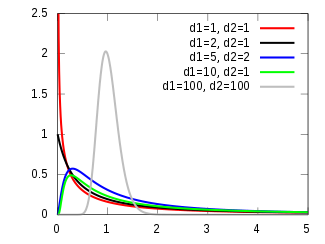
\includegraphics[scale=.5]{f}
	}{
		Suponga que la mitad de los hogares en un país tienen ingresos inferiores a \$ 50,000 y la otra mitad tienen ingresos superiores a \$ 50,000; esto indica que el ingreso familiar promedio es de \$ 50,000. Entre los hogares con ingresos inferiores a \$ 50,000, el valor más pequeño posible es \$ 0. Entre los hogares con ingresos superiores a \$ 50,000, puede haber ingresos de varios millones de dólares por año. Este desequilibrio entre los ingresos por debajo de la mediana y por encima de la mediana hace que la media sea sustancialmente más alta que la mediana. Supongamos, por ejemplo, que el ingreso promedio en este caso es de \$ 120,000. Esto muestra que la distribución de los ingresos familiares está sesgada positivamente.
	}{9cm}
	
	\subsection{Distribución Lognormal}
	
	\overview{
		mide eventos con comportamiento simétrico en el logaritmo de su variable
	}{
		$f(x)=\frac{1}{x\sigma \sqrt{2\pi}}e^{-\frac{(lnx-\mu)^2}{2\sigma^2}}$
	}{
		$F(x)=\frac{1}{2}+\frac{1}{2}erf[\frac{lnx-\mu}{\sqrt{2}\sigma}]$, erf es la función de error.
	}{
		$e^{\mu+\frac{\sigma ^2}{2}}$
	}{
		$(e^{\sigma^2}-1)e^{2\mu+\sigma^2}$
	}{
		En la hidrología la utilizan para analizar variables aleatorias continuas como los valores máximos de la precipitación y la descarga de ríos, y para describir el comportamientos de las épocas de sequía.
	}{
		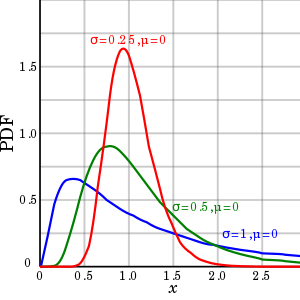
\includegraphics[scale=.5]{lognormal}
	}{
		Cuando se toman datos de frecuencia estos la mayoría de veces se comportan con una distribución lognormal. Se estudió una empresa la cual cumplía tener parámetros $\mu=4,\;\sigma=2$, como esto se puede obtener la probabilidad de que dicha empresa esté usando cierta cantidad de potencia (db por hora), en cualquier hora peculiar.
	}{9cm}

	\subsection{Distribución de Pareto}
	
	\overview{
		mide eventos que se distribuyen de una forma parecida al logaritmo.
	}{
		$\displaystyle f(x)=\frac{\alpha x_m^\alpha}{x^{\alpha+1}}$ $x>x_m$
	}{
		$F(x)=1-(\frac{x_m}{x})^\alpha$, $x\ge x_m$
	}{
		$\displaystyle\frac{\alpha x_m}{\alpha-1}$, $\alpha > 1$
	}{
		$\displaystyle\frac{x_m^2\alpha}{(\alpha-1)^2(\alpha-2)}$
	}{
		Es utilizada al igual que la lognormal en la hidrología para analizar variables aleatorias continuas como los valores máximos de la precipitación y la descarga de ríos, y para describir el comportamientos de las épocas de sequía.
	}{
		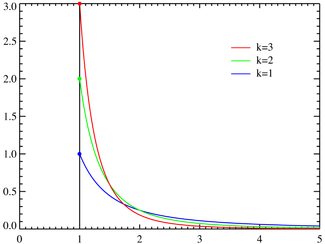
\includegraphics[scale=.5]{pareto}
	}{
		algunos ejemplos de utilización de esta distribución se da en: El tamaño de los asentamientos humanos, distribución del tamaño del archivo del tráfico de Internet, Tasas de error de la unidad de disco duro.
	}{9cm}

	\subsection{Distribución de Laplace}
	
	\overview{
		mide eventos que tienen distribución en forma de dos exponenciales adyacentes y con caras contrarias.
	}{
		$f(x)=\frac{1}{2b}e^{-\frac{|x-\mu|}{b}}$
	}{
		$F(x)=0.5e^{\frac{x-\mu}{b}}\;x\leq\mu,\quad F(x)=1-0.5e^{\frac{x-\mu}{b}}\;x\ge\mu$
	}{
		$\mu$
	}{
		$2b^2$
	}{
		Es utilizada al igual que la lognormal y de Pareto en la misma área con las mismas aplicaciones únicamente con la diferencia de como se ajustan.
	}{
		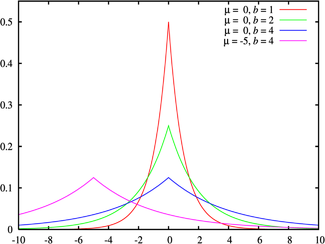
\includegraphics[scale=.5]{laplace}
	}{
		por ejemplo podemos utilizar la distribución de Laplace para el reconocimiento de voz y la compresión JPEG.
	}{9cm}

	\newpage
	
	\addtocounter{section}{1}
	\addcontentsline{toc}{section}{\thesection. \hspace{.002cm} Referencias}
	\bibliographystyle{apalike}
	\bibliography{bibliography}
	\nocite{*}
	
\end{document}